documentclass{article}
\usepackage{tikz}
\usetikzlibrary{positioning, shapes.geometric, shadows, arrows.meta}

\begin{document}

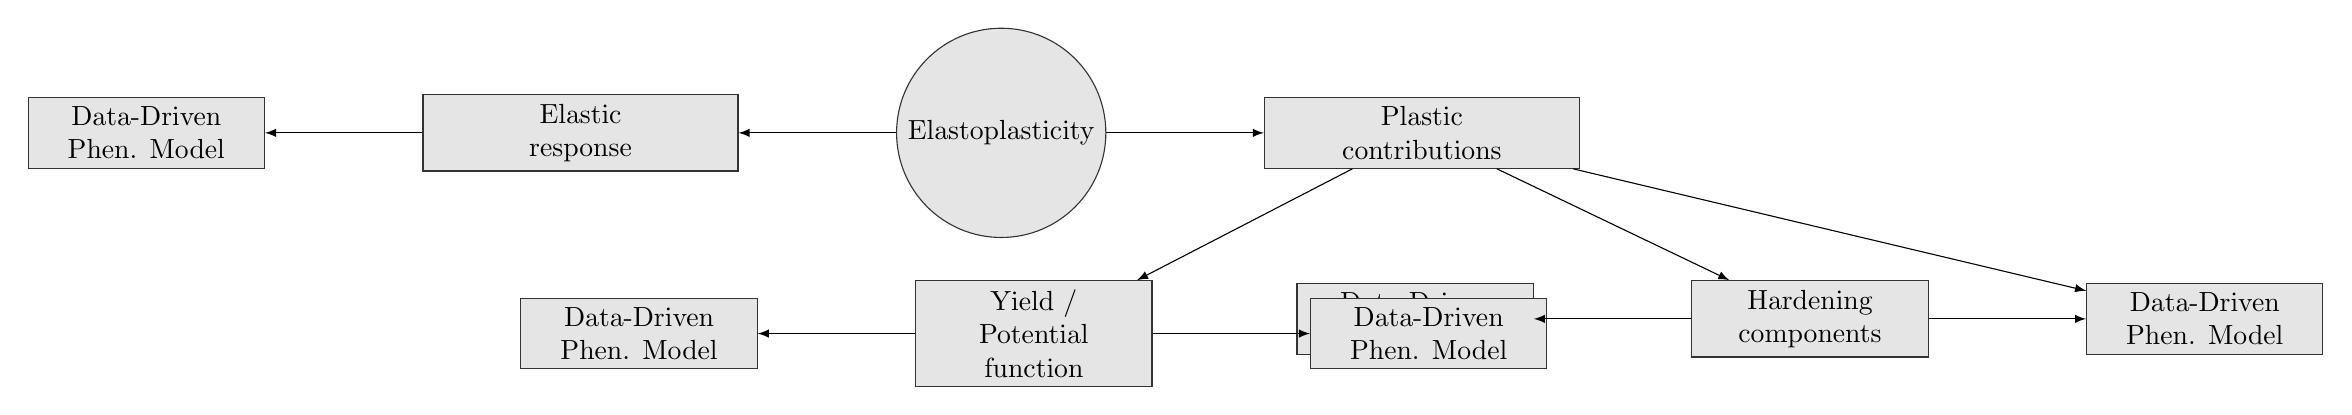
\begin{tikzpicture}[node distance = 2cm]
    \node[circle,draw=black!80,fill=gray!20, minimum size=0.5cm] (elasto_plasticity) {Elastoplasticity};
    \node[left=of elasto_plasticity,align=center,draw=black!80,fill=gray!20, minimum width=4cm] (elastic_response) {Elastic \\response};
    \node[right=of elasto_plasticity,align=center,draw=black!80,fill=gray!20, minimum width=4cm] (plastic_contributions) {Plastic \\contributions};
    \node[below left=of plastic_contributions,align=center,draw=black!80,fill=gray!20, minimum width=3cm] (yield_potential_function) {Yield / \\ Potential \\ function};
    \node[below right=of plastic_contributions,align=center,draw=black!80,fill=gray!20, minimum width=3cm] (hardening_components) {Hardening \\components};
    \node[right=of hardening_components,align=center,draw=black!80,fill=gray!20, minimum width=3cm] (flow_direction) {Flow \\direction};
    \node[left=of elastic_response,align=center,draw=black!80,fill=gray!20, minimum width=3cm] (data_driven_elasto_response) {Data-Driven \\ Phen. Model};
    \node[left=of yield_potential_function,align=center,draw=black!80,fill=gray!20, minimum width=3cm] (data_driven_yield_potential_function) {Data-Driven \\ Phen. Model};
    \node[left=of hardening_components,align=center,draw=black!80,fill=gray!20, minimum width=3cm] (data_driven_hardening_components) {Data-Driven \\ Phen. Model};
    \node[right=of yield_potential_function,align=center,draw=black!80,fill=gray!20, minimum width=3cm] (data_driven_yield_potential_function_right) {Data-Driven \\ Phen. Model};
    \node[right=of hardening_components,align=center,draw=black!80,fill=gray!20, minimum width=3cm] (data_driven_hardening_components_right) {Data-Driven \\ Phen. Model};

    \draw[-latex] (elasto_plasticity) -- (elastic_response);
    \draw[-latex] (elasto_plasticity) -- (plastic_contributions);
    \draw[-latex] (plastic_contributions) -- (yield_potential_function);
    \draw[-latex] (plastic_contributions) -- (hardening_components);
    \draw[-latex] (plastic_contributions) -- (flow_direction);

    \draw[-latex] (elastic_response) -- (data_driven_elasto_response);
    \draw[-latex] (yield_potential_function) -- (data_driven_yield_potential_function);
    \draw[-latex] (hardening_components) -- (data_driven_hardening_components);
    \draw[-latex] (yield_potential_function) -- (data_driven_yield_potential_function_right);
    \draw[-latex] (hardening_components) -- (data_driven_hardening_components_right);
\end{tikzpicture}

\end{document}